\section{Superconductivity}\label{sec:7.2}

Aluminum loses its electrical resistance below \SI{1.18}{K}, and at the lowest temperatures tunneling measures an energy gap of \SI{0.18}{meV} at its Fermi surface~\cite[Table~III]{savrasov1996electron}. Unlike a band gap, it opens because the electrons within a few tens of meV of the Fermi surface bind into pairs, and an excitation that conserves the number of electrons must break a pair, at a cost of $2\Delta_{\mathrm{BCS}} \approx \SI{0.36}{meV}$. This is the smallest quantum of \cref{tab:1-quanta}, and by the bound $m_{\mathrm{min}} = 2E_{\mathrm{th}}/v_{\mathrm{max}}^2$ of \cref{sec:1.3} it would let dark matter far below a keV deposit detectable energy (\cref{we:7-al})~\cite{hochberg2016detecting}. Superconducting films are also the sensors that read out most phonon-based detectors (\cref{sec:1.5}). Where does the attraction that binds the pairs come from, and how strong is it? What are the excitations of the paired state, and how do the density and the spin density of the electrons create them? And does the answer respect charge conservation, which the simplest treatment of the paired state does not? We start from the electron--phonon vertex of \cref{sec:6.2}.

\subsection{The phonon-mediated attraction}

Two electrons repel each other through the Coulomb interaction, yet in a metal they can attract each other by exchanging a phonon. \Cref{app:D.11} showed how. In the diagram rules, a phonon line replaces the Coulomb line, and with the normalization of \cref{eq:A.6-Hep}, in which the vertex $g$ comes with $1/\sqrt N$, the rule \cref{eq:D.11-boson} reads $-v_{\mathrm{C}}/\Vol \to -|g|^2\mathsf{D}_0(\vect{Q},\omega)/N$. Two electrons that exchange energy $\omega$ through a phonon $(\vect{Q},\nu)$ therefore feel the interaction
\begin{equation}
  \frac{1}{N}\,|g_\nu(\vect{k},\vect{Q})|^2\,\mathsf{D}_0(\vect{Q}\nu,\omega) = \frac{1}{N}\,\frac{2\omega_{\vect{Q}\nu}\,|g_\nu(\vect{k},\vect{Q})|^2}{\omega^2 - \omega_{\vect{Q}\nu}^2} ,
  \label{eq:7.2-Veff}
\end{equation}
with $g_\nu$ the vertex of a single band at the Fermi level, whose band indices we drop. For $|\omega| < \omega_{\vect{Q}\nu}$ it is negative, an attraction. The attraction is retarded. An electron moving through the crystal pulls the ions toward its path, and the ions, which respond on the scale $1/\omega_{\vect{Q}\nu}$, are still displaced after the electron has left. A second electron that arrives within that time is attracted by the positive charge the first one left behind. The screened Coulomb repulsion between the two acts only when they are close at the same moment, and by then the first electron is far away. Bardeen and Pines combined the two interactions in the electron gas and found the net interaction attractive for energy transfers below the phonon energy~\cite{bardeen1955electron}. In a scattering of two electrons near the Fermi surface the energy transfer is $\omega = \xi_{\vect{k}'} - \xi_{\vect{k}}$, with $\xi_{\vect{k}}$ the band energy measured from the Fermi level. The attraction acts between electrons whose energies lie within about the Debye frequency $\omega_{\mathrm{D}}$ of the Fermi surface, the scale of the largest phonon energies (\cref{sec:5.2}).

\paragraph{The pairing strength.} Take two electrons of opposite momentum and spin, $(\vect{k}\!\uparrow, -\vect{k}\!\downarrow)$, and let them scatter into $(\vect{k}'\!\uparrow, -\vect{k}'\!\downarrow)$ with $\vect{Q} = \vect{k}' - \vect{k}$. For energy transfers small compared with the phonon energy, \cref{eq:7.2-Veff} is its static value $-2|g_\nu|^2/(N\omega_{\vect{Q}\nu})$. In the interaction Hamiltonian $(1/2N)\sum_{\vect{Q}}v(\vect{Q})\,n_e(\vect{Q})n_e(-\vect{Q})$ the pair process appears twice, once with the spin-up electron in $n_e(\vect{Q})$ and once with the spin-down electron there, which cancels the $\frac12$. Time reversal makes the vertex of the spin-down electron, $g_\nu(-\vect{k},-\vect{Q})$, the complex conjugate of $g_\nu(\vect{k},\vect{Q})$, so the product of the two vertices is $|g_\nu(\vect{k},\vect{Q})|^2$. The pair term is therefore
\begin{equation*}
  -\frac{2}{N}\sum_\nu\frac{|g_\nu(\vect{k},\vect{Q})|^2}{\omega_{\vect{Q}\nu}}\;c^\dagger_{\vect{k}'\uparrow}c^\dagger_{-\vect{k}'\downarrow}c_{-\vect{k}\downarrow}c_{\vect{k}\uparrow} .
\end{equation*}
The model of Bardeen, Cooper and Schrieffer~\cite{bardeen1957theory} replaces the coefficient by a constant $-V_{\mathrm{BCS}}/\Vol$, with $\Vol = N\Omega$ the volume of the crystal and $\Omega$ the unit-cell volume, for all $\vect{k}$ and $\vect{k}'$ within $\omega_{\mathrm{D}}$ of the Fermi surface, and by zero outside that shell. The natural constant is the Fermi-surface average, $V_{\mathrm{BCS}} = 2\Omega\langle\sum_\nu|g_\nu|^2/\omega_{\vect{Q}\nu}\rangle_{\mathrm{FS}}$, where $\langle X\rangle_{\mathrm{FS}} = \sum_{\vect{k}\vect{k}'}X\,\delta(\xi_{\vect{k}})\delta(\xi_{\vect{k}'})/[\sum_{\vect{k}}\delta(\xi_{\vect{k}})]^2$ averages over both electrons on the Fermi surface. With $\sum_{\vect{k}}\delta(\xi_{\vect{k}}) = N\Omega\,\mathcal{N}_{\mathrm{F}}$ for one spin orientation and the Eliashberg function \cref{eq:6.4-a2F},
\begin{equation*}
  \mathcal{N}_{\mathrm{F}}V_{\mathrm{BCS}} = \frac{2}{\mathcal{N}_{\mathrm{F}}\Omega\,N^2}\sum_{\vect{k}\vect{Q}\nu}\frac{|g_\nu(\vect{k},\vect{Q})|^2}{\omega_{\vect{Q}\nu}}\,\delta(\xi_{\vect{k}})\,\delta(\xi_{\vect{k}+\vect{Q}}) = 2\int_0^\infty\dd\omega\,\frac{\alpha^2F(\omega)}{\omega} .
\end{equation*}
The right side is the coupling constant of \cref{eq:6.4-lambda}:
\begin{keyresult}[Phonon-mediated pairing strength]
\begin{equation}
  \mathcal{N}_{\mathrm{F}}V_{\mathrm{BCS}} = \lambda_{\mathrm{ep}} .
  \label{eq:7.2-NV}
\end{equation}
\end{keyresult}
The dimensionless strength of the attraction is the same number that enhances the electron mass and that the phonon linewidths of \cref{sec:6.4} measure.

\Cref{eq:7.2-NV} leaves out the Coulomb repulsion and the quasiparticle renormalization, both of the same order. The screened Coulomb repulsion acts at all energy transfers, while the attraction acts only within $\omega_{\mathrm{D}}$ of the Fermi surface. Its Fermi-surface average is reduced by this mismatch of time scales to the Coulomb pseudopotential $\mu^*_{\mathrm{C}}$ of \cref{app:E.9}, of order 0.1, which subtracts from $\lambda_{\mathrm{ep}}$. The pairing electrons are, in addition, the quasiparticles of \cref{sec:6.4}, with the residue $1/(1 + \lambda_{\mathrm{ep}})$. The Eliashberg equations contain both effects. At low frequencies the renormalization function of \cref{eq:E.9-Z} is $1 + \lambda_{\mathrm{ep}}$, the mass enhancement. If we go further and cut the frequency-dependent coupling \cref{eq:E.9-lambda} off at about $\omega_{\mathrm{D}}$, replacing it by $\lambda_{\mathrm{ep}}$ below and by zero above, the Eliashberg gap equation \cref{eq:E.9-Delta} reduces to the BCS one derived below, \cref{eq:7.2-gap}, written in Matsubara form, with the effective coupling
\begin{equation}
  \mathcal{N}_{\mathrm{F}}V_{\mathrm{BCS}} \simeq \frac{\lambda_{\mathrm{ep}} - \mu^*_{\mathrm{C}}}{1 + \lambda_{\mathrm{ep}}} .
  \label{eq:7.2-NVren}
\end{equation}
For aluminum, with $\lambda_{\mathrm{ep}} = 0.44$ and $\mu^*_{\mathrm{C}} = 0.12$, this is 0.22, half of \cref{eq:7.2-NV}. In practice the gap of a real superconductor is computed by solving the Eliashberg equations with the $\alpha^2F$ of \cref{sec:6.4}, which comes from density-functional perturbation theory and Wannier interpolation.

\paragraph{The reduced Hamiltonian.} The attraction scatters pairs of any total momentum, but pairs of zero total momentum have the most final states. For every $\vect{k}$ in the shell, every $\vect{k}'$ in the shell is a possible final state of the pair $(\vect{k}\!\uparrow, -\vect{k}\!\downarrow)$. A pair with total momentum $\vect{P} \ne 0$, by contrast, needs both $\vect{k}$ and $\vect{P} - \vect{k}$ in the shell, a condition that removes most of the phase space once $|\vect{P}|$ exceeds $\omega_{\mathrm{D}}/v_{\mathrm{F}}$. The \emph{reduced} BCS Hamiltonian keeps only the zero-momentum pairs:
\begin{equation}
  H_{\mathrm{BCS}} = \sum_{\vect{k}\sigma}\xi_{\vect{k}}\,c^\dagger_{\vect{k}\sigma}c_{\vect{k}\sigma} - \frac{V_{\mathrm{BCS}}}{\Vol}{\sum_{\vect{k}\vect{k}'}}'c^\dagger_{\vect{k}\uparrow}c^\dagger_{-\vect{k}\downarrow}c_{-\vect{k}'\downarrow}c_{\vect{k}'\uparrow} ,
  \label{eq:7.2-HBCS}
\end{equation}
with the prime restricting $|\xi_{\vect{k}}|$ and $|\xi_{\vect{k}'}|$ to less than $\omega_{\mathrm{D}}$. The pairs of finite momentum return when we ask how the paired state responds to a probe at wavevector $\vect{q}$.

\subsection{Cooper pairs and the BCS state}

\paragraph{Mean field.} The paired state follows from the mean-field theory of \cref{app:D.20}. Define the pair amplitude $b_{\vect{k}} = \langle c_{-\vect{k}\downarrow}c_{\vect{k}\uparrow}\rangle$, which is zero in any state with a definite number of electrons, and the gap
\begin{equation}
  \Delta_{\mathrm{BCS}} = \frac{V_{\mathrm{BCS}}}{\Vol}{\sum_{\vect{k}}}'b_{\vect{k}} ,
  \label{eq:7.2-Delta}
\end{equation}
real by the choice of an overall phase. In \cref{eq:7.2-HBCS} each pair operator interacts with all $\sim N$ others with a strength of order $1/\Vol$, and replacing their sum by its average, \cref{eq:7.2-Delta}, makes an error that vanishes as $\Vol \to \infty$. The interaction then becomes the pair field $-\Delta_{\mathrm{BCS}}(c^\dagger_{\vect{k}\uparrow}c^\dagger_{-\vect{k}\downarrow} + c_{-\vect{k}\downarrow}c_{\vect{k}\uparrow})$ acting on each pair of modes, and for each $\vect{k}$ the mean-field Hamiltonian $H_{\mathrm{MF}}$ is the two-mode fermion problem \cref{eq:C.7-Hfermion} with $\xi_0 = \xi_{\vect{k}}$ and $g_0 = \Delta_{\mathrm{BCS}}$. It is diagonalized by the fermionic Bogoliubov transformation of \cref{app:C.7}, the counterpart of the bosonic one that diagonalized the antiferromagnet in \cref{sec:7.1}, with sines and cosines in place of hyperbolic functions. The quasiparticle operators are
\begin{equation}
  \gamma_{\vect{k}1} = u^{\mathrm{B}}_{\vect{k}}\,c_{\vect{k}\uparrow} - v^{\mathrm{B}}_{\vect{k}}\,c^\dagger_{-\vect{k}\downarrow}, \qquad
  \gamma_{\vect{k}2} = u^{\mathrm{B}}_{\vect{k}}\,c_{-\vect{k}\downarrow} + v^{\mathrm{B}}_{\vect{k}}\,c^\dagger_{\vect{k}\uparrow} ,
  \label{eq:7.2-gamma}
\end{equation}
and by \cref{eq:C.7-Efermion},
\begin{keyresult}[Bogoliubov quasiparticles]
\begin{equation}
  \begin{gathered}
  H_{\mathrm{MF}} = {\sum_{\vect{k}}}'E_{\vect{k}}\bigl(\gamma^\dagger_{\vect{k}1}\gamma_{\vect{k}1} + \gamma^\dagger_{\vect{k}2}\gamma_{\vect{k}2}\bigr) + \text{const}, \qquad
  E_{\vect{k}} = \bigl(\xi_{\vect{k}}^2 + \Delta_{\mathrm{BCS}}^2\bigr)^{1/2}, \\
  (u^{\mathrm{B}}_{\vect{k}})^2 = \frac12\Bigl(1 + \frac{\xi_{\vect{k}}}{E_{\vect{k}}}\Bigr), \qquad
  (v^{\mathrm{B}}_{\vect{k}})^2 = \frac12\Bigl(1 - \frac{\xi_{\vect{k}}}{E_{\vect{k}}}\Bigr), \qquad
  2u^{\mathrm{B}}_{\vect{k}}v^{\mathrm{B}}_{\vect{k}} = \frac{\Delta_{\mathrm{BCS}}}{E_{\vect{k}}} .
  \end{gathered}
  \label{eq:7.2-E}
\end{equation}
\end{keyresult}
The coefficients $u^{\mathrm{B}}_{\vect{k}}$ and $v^{\mathrm{B}}_{\vect{k}}$ are the \emph{coherence factors} of the BCS state. The quasiparticle $\gamma^\dagger_{\vect{k}1}$ carries momentum $\vect{k}$ and spin up. Far above the Fermi surface $u^{\mathrm{B}}_{\vect{k}} \to 1$ and it is an added electron; far below, $v^{\mathrm{B}}_{\vect{k}} \to 1$ and it is a removed electron of momentum $-\vect{k}$ and spin down, a hole; at the Fermi surface it is half of each, with energy $\Delta_{\mathrm{BCS}}$. The ground state, annihilated by every $\gamma$, is the BCS state
\begin{equation}
  |\mathrm{BCS}\rangle = \prod_{\vect{k}}\bigl(u^{\mathrm{B}}_{\vect{k}} + v^{\mathrm{B}}_{\vect{k}}\,c^\dagger_{\vect{k}\uparrow}c^\dagger_{-\vect{k}\downarrow}\bigr)|0\rangle ,
  \label{eq:7.2-BCS}
\end{equation}
in which each pair state $(\vect{k}\!\uparrow, -\vect{k}\!\downarrow)$ is occupied with probability $(v^{\mathrm{B}}_{\vect{k}})^2$. The step of the Fermi sea is smeared over an energy $\Delta_{\mathrm{BCS}}$, and the coherent superposition of empty and full pair states is what makes $b_{\vect{k}} = u^{\mathrm{B}}_{\vect{k}}v^{\mathrm{B}}_{\vect{k}}$ nonzero. The state $|\mathrm{BCS}\rangle$ has no definite electron number. Its relative number fluctuations are of order $N^{-1/2}$. They are negligible for energies but spoil the density response, which the last subsection repairs.

\paragraph{Quasiparticle density of states.} Since $\dd E_{\vect{k}}/\dd\xi_{\vect{k}} = \xi_{\vect{k}}/E_{\vect{k}}$, each energy $E > \Delta_{\mathrm{BCS}}$ is reached from two values of $\xi$, an electronlike state above the Fermi level and a holelike one below. With $\mathcal{N}_{\mathrm{F}}$ constant over the shell, the quasiparticles of one spin orientation have the density of states per volume
\begin{equation}
  \mathcal{N}_{\mathrm{qp}}(E) = 2\mathcal{N}_{\mathrm{F}}\,\frac{E}{\sqrt{E^2 - \Delta_{\mathrm{BCS}}^2}}\,\Theta(E - \Delta_{\mathrm{BCS}}) .
  \label{eq:7.2-dos}
\end{equation}
The factor 2 counts the two branches, not the spin; both spin orientations together have $g_{\mathrm{deg}}\mathcal{N}_{\mathrm{qp}}$, with $g_{\mathrm{deg}} = 2$. In the normal metal, $\mathcal{N}_{\mathrm{qp}} \to 2\mathcal{N}_{\mathrm{F}}$, the density of electron and hole excitations at energy $E$ above the ground state. Pairing removes the states from $|E| < \Delta_{\mathrm{BCS}}$ and piles them up at the edge, where the density diverges as $(E - \Delta_{\mathrm{BCS}})^{-1/2}$ (\cref{fig:7-bcs}a). The number of states is conserved: $\int_{\Delta_{\mathrm{BCS}}}^{\omega}\dd E\,\mathcal{N}_{\mathrm{qp}} = 2\mathcal{N}_{\mathrm{F}}(\omega^2 - \Delta_{\mathrm{BCS}}^2)^{1/2}$, which approaches the normal-state count $2\mathcal{N}_{\mathrm{F}}\omega$ as $\omega$ grows.

\paragraph{The gap equation.} The gap must reproduce itself through \cref{eq:7.2-Delta}. In thermal equilibrium the quasiparticles are independent fermions, occupied with $n_{\mathrm{F}}(E_{\vect{k}})$, and inverting \cref{eq:7.2-gamma} yields $b_{\vect{k}} = u^{\mathrm{B}}_{\vect{k}}v^{\mathrm{B}}_{\vect{k}}[1 - 2n_{\mathrm{F}}(E_{\vect{k}})] = (\Delta_{\mathrm{BCS}}/2E_{\vect{k}})\tanh(E_{\vect{k}}/2T)$. Inserting this, dividing by $\Delta_{\mathrm{BCS}}$ and replacing $\Vol^{-1}\sum_{\vect{k}}$ by $\mathcal{N}_{\mathrm{F}}\int\dd\xi$,
\begin{keyresult}[BCS gap equation and its weak-coupling solutions]
\begin{equation}
  \begin{gathered}
  \frac{1}{\mathcal{N}_{\mathrm{F}}V_{\mathrm{BCS}}} = \int_0^{\omega_{\mathrm{D}}}\dd\xi\,\frac{\tanh\bigl(\sqrt{\xi^2 + \Delta_{\mathrm{BCS}}^2}/2T\bigr)}{\sqrt{\xi^2 + \Delta_{\mathrm{BCS}}^2}} , \\
  \Delta_{\mathrm{BCS}}(0) \simeq 2\omega_{\mathrm{D}}\,\ee^{-1/\mathcal{N}_{\mathrm{F}}V_{\mathrm{BCS}}}, \qquad
  T_c = \frac{2\ee^{\gamma_{\mathrm{E}}}}{\pi}\,\omega_{\mathrm{D}}\,\ee^{-1/\mathcal{N}_{\mathrm{F}}V_{\mathrm{BCS}}}, \\
  \frac{\Delta_{\mathrm{BCS}}(0)}{T_c} = \pi\ee^{-\gamma_{\mathrm{E}}} = 1.764 ,
  \end{gathered}
  \label{eq:7.2-gap}
\end{equation}
\end{keyresult}
with $\gamma_{\mathrm{E}} = 0.5772$ Euler's constant. The right side of the gap equation diverges logarithmically as $\Delta_{\mathrm{BCS}}$ and $T$ go to zero, which is why a solution exists for any attraction. A weak attraction does not bind two particles in three-dimensional vacuum, where the density of pair states vanishes as $\xi^{1/2}$ and the integral converges; above a Fermi surface that density stays finite down to zero energy. At $T = 0$ the integral is $\operatorname{arsinh}(\omega_{\mathrm{D}}/\Delta_{\mathrm{BCS}})$, and the gap follows; at $T_c$ the gap closes, and the integral, evaluated in \cref{app:D.20} by expanding the hyperbolic tangent over Matsubara frequencies, fixes the critical temperature. The gap is nonanalytic in the coupling and invisible at any finite order of perturbation theory. Both $\Delta_{\mathrm{BCS}}(0)$ and $T_c$ depend exponentially on $\mathcal{N}_{\mathrm{F}}V_{\mathrm{BCS}}$ and linearly on the cutoff, but their ratio depends on neither, and it is the same for every material within the model. Deviations from 1.764 measure the strength and the retardation of the real interaction. Aluminum, with the measured \SI{0.18}{meV} and \SI{1.18}{K}, has $2\Delta_{\mathrm{BCS}}/T_c = 3.54$, against $2\pi\ee^{-\gamma_{\mathrm{E}}} = 3.53$.

\paragraph{The pair-breaking threshold.} A dark-matter particle or a phonon couples to the electrons through operators that conserve their number, such as the density $n_e(\vect{q})$ and the spin density. Expressed through \cref{eq:7.2-gamma}, such an operator either scatters a quasiparticle that is already present or creates two at once, one from each branch; it never creates a single one, which would change the electron number by one. At $T = 0$ no quasiparticles are present, and the lowest excitation that a probe can make is a pair, at
\begin{equation}
  \omega \ge E_{\vect{k}} + E_{\vect{k}+\vect{q}} \ge 2\Delta_{\mathrm{BCS}} ,
  \label{eq:7.2-threshold}
\end{equation}
the \emph{pair-breaking threshold}. It is reached when both quasiparticles lie at the Fermi surface, which for $q < 2k_{\mathrm{F}}$ is always possible. In the language of \cref{sec:1.3}, $E_{\mathrm{th}} = 2\Delta_{\mathrm{BCS}}$. At $T > 0$ thermally excited quasiparticles can absorb energy in smaller amounts, but their number is suppressed by $\ee^{-\Delta_{\mathrm{BCS}}/T}$, and in aluminum at \SI{10}{mK} the exponent is $-208$.

\begin{figure}[t]
  \centering
  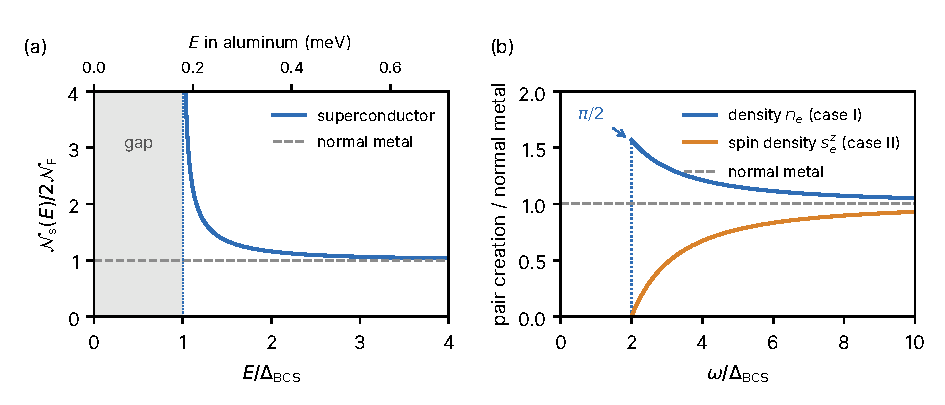
\includegraphics[width=\linewidth]{figures/ch07/fig7_2.pdf}
  \caption{Quasiparticles of a BCS superconductor at $T = 0$. (a) Density of states per spin orientation, \cref{eq:7.2-dos}, in units of its normal-state value $2\mathcal{N}_{\mathrm{F}}$: no states below $\Delta_{\mathrm{BCS}}$ (gray), an integrable divergence at the edge. The top axis shows the energy for aluminum, $\Delta_{\mathrm{BCS}} = 1.764\,T_c = \SI{0.179}{meV}$ with the measured $T_c = \SI{1.18}{K}$. (b) Rate of pair creation by a probe of energy $\omega$ coupled to the electron density (case I) or to the $z$ component of the spin density (case II), divided by its normal-state value, \cref{eq:7.2-pairspec}. Both are bare quasiparticle bubbles for a linearized band with $q \ll k_{\mathrm{F}}$ and $qv_{\mathrm{F}} \ge \omega$, the regime of dark-matter scattering in aluminum, where the ratio does not depend on $q$. The density curve jumps to $\pi/2$ at the threshold $2\Delta_{\mathrm{BCS}}$; the spin curve starts from zero and is the zero-temperature conductivity ratio of Mattis and Bardeen. Both tend to one for $\omega \gg \Delta_{\mathrm{BCS}}$.}
  \label{fig:7-bcs}
\end{figure}

\subsection{Coherence factors}

The amplitude to break a pair depends on what the probe couples to, because each quasiparticle is part electron and part hole and the two parts can interfere. Take the density, $n_e(\vect{q}) = \sum_{\vect{k}\sigma}c^\dagger_{\vect{k}+\vect{q},\sigma}c_{\vect{k}\sigma}$, and the $z$ component of the spin density of \cref{eq:7.1-se}, $s^z_e(\vect{q}) = \frac12\sum_{\vect{k}}(c^\dagger_{\vect{k}+\vect{q}\uparrow}c_{\vect{k}\uparrow} - c^\dagger_{\vect{k}+\vect{q}\downarrow}c_{\vect{k}\downarrow})$. Write $u = u^{\mathrm{B}}_{\vect{k}}$, $v = v^{\mathrm{B}}_{\vect{k}}$, and primes for $\vect{k}' = \vect{k} + \vect{q}$. Substituting the inverse of \cref{eq:7.2-gamma} into the spin-up term gives $c^\dagger_{\vect{k}'\uparrow}c_{\vect{k}\uparrow} = u'u\,\gamma^\dagger_{\vect{k}'1}\gamma_{\vect{k}1} + u'v\,\gamma^\dagger_{\vect{k}'1}\gamma^\dagger_{\vect{k}2} + \dots$, and the spin-down term, after relabeling $\vect{k} \to -\vect{k} - \vect{q}$, contributes to the same two processes with $-vv'$ and $uv'$ (\cref{app:D.20}). The density adds the spin-up and spin-down terms and the spin density subtracts them, so that the amplitudes are
\begin{equation}
  \begin{aligned}
  n_e(\vect{q}):&\quad \text{pair creation } u'v + v'u, \qquad \text{quasiparticle scattering } uu' - vv' ,\\
  s^z_e(\vect{q}):&\quad \text{pair creation } \tfrac12(u'v - v'u), \qquad \text{quasiparticle scattering } \tfrac12(uu' + vv') .
  \end{aligned}
  \label{eq:7.2-coh}
\end{equation}
Squared and expressed through the energies with \cref{eq:7.2-E},
\begin{keyresult}[Coherence factors of pair creation and quasiparticle scattering]
\begin{equation}
  (uv' \pm vu')^2 = \frac12\Bigl(1 - \frac{\xi\xi' \mp \Delta_{\mathrm{BCS}}^2}{EE'}\Bigr), \qquad
  (uu' \mp vv')^2 = \frac12\Bigl(1 + \frac{\xi\xi' \mp \Delta_{\mathrm{BCS}}^2}{EE'}\Bigr) ,
  \label{eq:7.2-cohE}
\end{equation}
\end{keyresult}
with the upper signs for the density and the lower signs for the spin density. The two operators differ in their behavior under time reversal: the density is even and the spin density odd. These are the two classes that Tinkham calls case~I and case~II~\cite{tinkham2004introduction}. Every one-body probe is a sum of a part even and a part odd under time reversal, one from each class; the current, which drives the absorption of light, is odd and belongs to case~II with the spin.

At the threshold both quasiparticles lie at the Fermi surface, $\xi = \xi' = 0$, and the creation factor is $\frac12(1 \pm 1)$: one for the density, zero for the spin density. In the density the electron and hole parts of the pair add; in the spin density they cancel. Away from the Fermi surface the factors depend on the signs of $\xi$ and $\xi'$, and the dark-matter kinematics decide how these are sampled. For a linearized band, $\xi' = \xi + v_{\mathrm{F}}q\cos\theta$ with $\theta$ the angle between $\vect{k}$ and $\vect{q}$. Two quasiparticles with $E + E' = \omega$ have $|\xi'- \xi| \le |\xi| + |\xi'| < \omega$, so as long as $v_{\mathrm{F}}q \ge \omega$ every pair of values $(\xi, \xi')$ in that range is reached at some angle. Since $\cos\theta$ is uniformly distributed over the Fermi sphere, each pair is reached with the same weight.

This is the regime of dark-matter scattering in a metal. A dark-matter particle that deposits $\omega$ transfers at least $q = \omega/v_{\mathrm{max}}$ (\cref{sec:1.3}), and in aluminum $v_{\mathrm{F}} = \num{6.75e-3}$, the free-electron value of \cref{sec:6.4}, is 2.5 times $v_{\mathrm{max}}$. Then $\xi$ and $\xi'$ are independent and uniformly distributed, and the terms odd in either one average to zero. The mean creation factor of the density becomes $\frac12(1 + \Delta_{\mathrm{BCS}}^2/EE')$, and that of the spin density $\frac12(1 - \Delta_{\mathrm{BCS}}^2/EE')$.

\paragraph{The pair-creation spectrum.} With these factors the absorption spectrum of the paired state follows in closed form. At $T = 0$ the dynamic structure factor of the density is the golden-rule sum over pairs, $S(\vect{q},\omega) = (2\pi/\Vol)\sum_{\vect{k}}(uv' + vu')^2\,\delta(\omega - E_{\vect{k}} - E_{\vect{k}+\vect{q}})$; the sum over $\vect{k}$ with both branches covers both spin orientations, as the normal limit below confirms. Replace $\Vol^{-1}\sum_{\vect{k}}$ by $\mathcal{N}_{\mathrm{F}}\int\dd\xi\int_{-1}^1\dd\!\cos\theta/2$, trade the angle for $\xi'$ at $\dd\xi'/2v_{\mathrm{F}}q$, and change variables from $\xi$ and $\xi'$ to $E$ and $E'$ with the density of states \cref{eq:7.2-dos} for each, which absorbs the sum over the four sign combinations. In the normal state, $\Delta_{\mathrm{BCS}} = 0$, the result is $S_{\mathrm{n}}(\vect{q},\omega) = 2\pi\mathcal{N}_{\mathrm{F}}\,\omega/v_{\mathrm{F}}q = m_e^2\omega/\pi q$, the electron gas of \cref{sec:4.5} below its curve $\omega = qv_{\mathrm{F}} - q^2/2m_e$. In the superconductor,
\begin{keyresult}[Bare pair-creation spectra for $qv_{\mathrm{F}} \ge \omega$]
\begin{equation}
  \frac{S_{\mathrm{I,II}}(\vect{q},\omega)}{S_{\mathrm{n}}(\vect{q},\omega)} = \frac{1}{\omega}\int_{\Delta_{\mathrm{BCS}}}^{\omega - \Delta_{\mathrm{BCS}}}\dd E\,\frac{E(\omega - E) \pm \Delta_{\mathrm{BCS}}^2}{\sqrt{E^2 - \Delta_{\mathrm{BCS}}^2}\,\sqrt{(\omega - E)^2 - \Delta_{\mathrm{BCS}}^2}}\;\Theta(\omega - 2\Delta_{\mathrm{BCS}}) ,
  \label{eq:7.2-pairspec}
\end{equation}
\end{keyresult}
with the upper sign for the density (case~I) and the lower sign for the spin density (case~II), each divided by its own normal-state value. \Cref{fig:7-bcs}(b) shows both. Near the threshold $E(\omega - E) \to \Delta_{\mathrm{BCS}}^2$, so the numerator of the integrand tends to $\Delta_{\mathrm{BCS}}^2 \pm \Delta_{\mathrm{BCS}}^2$, that is $2\Delta_{\mathrm{BCS}}^2$ for the density and zero for the spin density, while the denominator tends to $2\Delta_{\mathrm{BCS}}$ times the product of the two edge divergences of \cref{eq:7.2-dos}. The integral of that product over the shrinking interval stays finite, $\int\dd E\,[(E - \Delta_{\mathrm{BCS}})(\omega - \Delta_{\mathrm{BCS}} - E)]^{-1/2} = \pi$. For the density the integral is therefore $\Delta_{\mathrm{BCS}}\pi$, and with the prefactor $1/\omega = 1/2\Delta_{\mathrm{BCS}}$ the spectrum jumps at $\omega = 2\Delta_{\mathrm{BCS}}$ to $\pi/2$ times the normal value. Since $E(\omega - E) - \Delta^2_{\mathrm{BCS}}$ vanishes at the threshold, the spin spectrum instead rises continuously from zero. Far above the gap both approach the normal metal: at $\omega = 4\Delta_{\mathrm{BCS}}$ the ratios are 1.21 and 0.67. The case-II integral is the one that Mattis and Bardeen found for the absorption of light by a superconductor at zero temperature~\cite{mattis1958theory}, in the limit of short mean free path, where $\xi$ and $\xi'$ are again independent, and it reproduces their closed form in elliptic integrals. For a dark-matter particle that couples to the electron density, the gap therefore enhances the bare rate just above threshold instead of suppressing it. The pile-up of states at the edge outweighs the narrow window of energies.

Quasiparticle scattering, the second process in \cref{eq:7.2-coh}, needs quasiparticles in the initial state. It is weighted by $n_{\mathrm{F}}(E)[1 - n_{\mathrm{F}}(E')]$ and absorbs energies below $2\Delta_{\mathrm{BCS}}$. Its coherence factors are the mirror images of the creation factors: the density scattering factor averages to $\frac12(1 - \Delta_{\mathrm{BCS}}^2/EE')$ and vanishes at the edge, which is why the attenuation of sound in a superconductor falls with temperature as $2n_{\mathrm{F}}(\Delta_{\mathrm{BCS}})$ instead of showing the pile-up~\cite{tinkham2004introduction}. In a detector at millikelvin temperatures this channel is closed by the factor $\ee^{-\Delta_{\mathrm{BCS}}/T}$.

\Cref{eq:7.2-pairspec} for the density is the bare quasiparticle bubble, the response of independent Bogoliubov quasiparticles, and not yet the density response of the superconductor.

\subsection{Charge conservation and the Nambu formalism}

At $\vect{q} = 0$ the density is the total electron number $\op{N}_e$, which commutes with \cref{eq:7.2-HBCS} and cannot excite anything. Yet by \cref{eq:7.2-coh} its pair-creation amplitude at $\vect{q} = 0$ is $2uv = \Delta_{\mathrm{BCS}}/E_{\vect{k}}$, not zero. The error comes from the mean field. $H_{\mathrm{MF}}$ creates and destroys pairs, so it does not commute with $\op{N}_e$, and its eigenstates have no definite electron number. A response computed from independent quasiparticles then puts spectral weight $\Delta_{\mathrm{BCS}}^2/E_{\vect{k}}^2$ at $\omega = 2E_{\vect{k}}$ into the uniform density response. Its first moment, by the gap equation at $T = 0$, $\Vol^{-1}\sum'_{\vect{k}}1/E_{\vect{k}} = 2/V_{\mathrm{BCS}}$, is
\begin{equation}
  \int_0^\infty\dd\omega\,\omega\,S^0(0,\omega) = \frac{4\pi}{\Vol}{\sum_{\vect{k}}}'\frac{\Delta_{\mathrm{BCS}}^2}{E_{\vect{k}}} = \frac{8\pi\Delta_{\mathrm{BCS}}^2}{V_{\mathrm{BCS}}} .
  \label{eq:7.2-violation}
\end{equation}
All bubbles here carry the restriction of the pair states to the shell, as in \cref{eq:7.2-HBCS}. The f-sum rule \cref{eq:4.3-fsum} requires $\pi\nd_eq^2/m_e$, which vanishes at $q = 0$. The bare bubble violates it, and not only at $q = 0$: as long as $v_{\mathrm{F}}q \ll \omega_{\mathrm{D}}$ the spurious first moment keeps the value \cref{eq:7.2-violation}, since it comes from pairs spread over the whole shell, at frequencies up to $2\omega_{\mathrm{D}}$. For a linearized band the moment stays within \SI{0.2}{\percent} of this value up to $v_{\mathrm{F}}q = 20\Delta_{\mathrm{BCS}}$. With $\nd_e = \frac43\mathcal{N}_{\mathrm{F}}E_{\mathrm{F}}$ for free electrons, the spurious moment relative to the f-sum is $12(\Delta_{\mathrm{BCS}}/v_{\mathrm{F}}q)^2/\mathcal{N}_{\mathrm{F}}V_{\mathrm{BCS}}$, which exceeds one for $v_{\mathrm{F}}q < 8.6\,\Delta_{\mathrm{BCS}}$ at the aluminum coupling $\mathcal{N}_{\mathrm{F}}V_{\mathrm{BCS}} = 0.164$ of \cref{we:7-al}, obtained with a \SI{40}{meV} cutoff. The bare bubble is a poor guide to the total spectral weight even at the momenta of dark-matter scattering.

\paragraph{Nambu form.} The cure is easiest to see in the notation of Nambu~\cite{nambu1960quasi}, which treats the two operators that pairing mixes as one spinor, $\Psi_{\vect{k}} = (c_{\vect{k}\uparrow}, c^\dagger_{-\vect{k}\downarrow})^{\mathrm{T}}$. Bilinears $O_A(\vect{q}) = \sum_{\vect{k}}\Psi^\dagger_{\vect{k}+\vect{q}}A\,\Psi_{\vect{k}}$ with the $2\times2$ matrices
\begin{equation}
  \boldsymbol{\eta} = \begin{pmatrix}1 & 0\\ 0 & -1\end{pmatrix}, \qquad
  \mathsf{s}_1 = \begin{pmatrix}0 & 1\\ 1 & 0\end{pmatrix}, \qquad
  \mathsf{s}_2 = \begin{pmatrix}0 & -\ii\\ \ii & 0\end{pmatrix}
  \label{eq:7.2-nambu}
\end{equation}
are the physical operators: $O_{\boldsymbol{\eta}}(\vect{q}) = n_e(\vect{q})$ for $\vect{q} \ne 0$, after anticommuting the spin-down term, while $O_{\mathsf{s}_1}$ and $O_{\mathsf{s}_2}$ create and destroy pairs of total momentum $\vect{q}$ (\cref{app:D.21}). For a real gap, $\mathsf{s}_1$ changes the magnitude of the pair field and $\mathsf{s}_2$ its phase. The matrix $\boldsymbol{\eta}$ is the one of \cref{app:C.7}; the three matrices obey the algebra of the Pauli matrices, which we do not call $\sigma_i$ because those act on the electron spin. In this notation $H_{\mathrm{MF}} = \sum_{\vect{k}}\Psi^\dagger_{\vect{k}}h_{\vect{k}}\Psi_{\vect{k}} + \text{const}$ with $h_{\vect{k}} = \xi_{\vect{k}}\boldsymbol{\eta} - \Delta_{\mathrm{BCS}}\mathsf{s}_1$, whose eigenvalues are $\pm E_{\vect{k}}$, and the Matsubara Green's function of \cref{sec:4.7} becomes the $2\times2$ matrix $\GF_0(\vect{k},\ii\omega^{\mathrm{F}}) = (\ii\omega^{\mathrm{F}} - h_{\vect{k}})^{-1}$, whose off-diagonal elements are the pair amplitudes. The bare bubble with vertices $A$ and $B$ is the loop of \cref{sec:4.8} with a trace over the Nambu index, and the trace for $A = B = \boldsymbol{\eta}$ reproduces the case-I factor of \cref{eq:7.2-cohE}.

Since $[\mathsf{s}_1, \boldsymbol{\eta}] = -2\ii\mathsf{s}_2$,
\begin{equation}
  [H_{\mathrm{MF}}, n_e(\vect{q})] = \vect{q}\cdot\vect{j}_e(\vect{q}) + 2\ii\Delta_{\mathrm{BCS}}\,O_{\mathsf{s}_2}(\vect{q}) .
  \label{eq:7.2-comm}
\end{equation}
The kinetic term gives the current of the continuity equation \cref{eq:4.3-continuity}, and the pair field adds a term that turns density into fluctuations of the pair phase. Under $H_{\mathrm{MF}}$, charge leaks into the condensate and does not come back. The full Hamiltonian has no such term, because the attraction $-V_{\mathrm{BCS}}\psi^\dagger_\uparrow\psi^\dagger_\downarrow\psi_\downarrow\psi_\uparrow$ is a function of the local densities and commutes with $n_e(\vect{q})$, up to corrections of relative order $v_{\mathrm{F}}q/\omega_{\mathrm{D}}$ from the shell (\cref{app:D.21}).

\paragraph{The conserving response.} The bare bubble misses that the pair field is itself made of electrons. A density perturbation at wavevector $\vect{q}$ changes the pair amplitudes, and the changed amplitudes act back on the quasiparticles as a pair field oscillating at $\vect{q}$ and $\omega$. Anderson~\cite{anderson1958random} included this as the linear response of the time-dependent mean field. To let the pair field respond at $\vect{q}$, the attraction must scatter pairs of every total momentum, not only the zero-momentum pairs of \cref{eq:7.2-HBCS}; written in the pair channels it is $-(V_{\mathrm{BCS}}/4\Vol)\sum_{\vect{P}}\sum_{a=1,2}O_{\mathsf{s}_a}(\vect{P})O_{\mathsf{s}_a}(-\vect{P})$ plus one-body terms. Its mean field at wavevector $\vect{q}$ couples the induced $\delta\langle O_{\mathsf{s}_a}\rangle$ back to $O_{\mathsf{s}_a}$. The response is then the random-phase approximation of \cref{sec:4.5}, with the pair channels $(\boldsymbol{\eta}, \mathsf{s}_1, \mathsf{s}_2)$ in place of the Coulomb channel and the kernel $K = \operatorname{diag}(0, -V_{\mathrm{BCS}}/2, -V_{\mathrm{BCS}}/2)$:
\begin{keyresult}[Conserving density response]
\begin{equation}
  R = R^0 + R^0KR, \qquad
  R_{\boldsymbol{\eta}\boldsymbol{\eta}} = R^0_{\boldsymbol{\eta}\boldsymbol{\eta}} + \sum_{a,b=1,2}R^0_{\boldsymbol{\eta}\mathsf{s}_a}\Bigl[\bigl(1 - KR^0\bigr)^{-1}K\Bigr]_{ab}R^0_{\mathsf{s}_b\boldsymbol{\eta}} ,
  \label{eq:7.2-Rc}
\end{equation}
\end{keyresult}
with the bare Nambu bubbles $R^0_{AB}$ and the inverse taken in the block of the two pair channels. In diagrams the correction is the bare bubble with a ladder of pair propagators between its two vertices. That it conserves charge follows from a general property of mean-field dynamics (\cref{app:D.21}). In a state for which Wick's theorem holds, the time derivative of any one-body average computed with the self-consistent mean field equals the one computed with the full Hamiltonian, and the full Hamiltonian obeys the continuity equation. The term $2\ii\Delta_{\mathrm{BCS}}\,\delta\langle O_{\mathsf{s}_2}\rangle$ that \cref{eq:7.2-comm} produces is cancelled by the commutator of $n_e$ with the induced pair field. A response that obeys the continuity equation satisfies the f-sum rule by the double-commutator argument of \cref{sec:4.3}.

At $\vect{q} = 0$ the cancellation can be seen in closed form. If the density of states is symmetric about the Fermi level over the shell, the bubbles that connect $\mathsf{s}_1$ to $\boldsymbol{\eta}$ or to $\mathsf{s}_2$ are odd in $\xi$ and vanish, and the magnitude of the pair field decouples. We assume this particle--hole symmetry here; real metals break it weakly, and the general argument above does not need it. The remaining bubbles are, with $F(\omega) = \Vol^{-1}\sum'_{\vect{k}}[E_{\vect{k}}(\omega^2 - 4E_{\vect{k}}^2)]^{-1}$,
\begin{equation}
  R^0_{\boldsymbol{\eta}\boldsymbol{\eta}} = 4\Delta_{\mathrm{BCS}}^2F, \qquad
  R^0_{\mathsf{s}_2\mathsf{s}_2} = \omega^2F - \frac{2}{V_{\mathrm{BCS}}}, \qquad
  R^0_{\mathsf{s}_2\boldsymbol{\eta}} = -R^0_{\boldsymbol{\eta}\mathsf{s}_2} = 2\ii\Delta_{\mathrm{BCS}}\,\omega F ,
  \label{eq:D.21-q0}
\end{equation}
where the gap equation was used in $R^0_{\mathsf{s}_2\mathsf{s}_2}$ (\cref{app:D.21}). The phase channel has the denominator $1 + \frac12V_{\mathrm{BCS}}R^0_{\mathsf{s}_2\mathsf{s}_2} = \frac12V_{\mathrm{BCS}}\omega^2F$, and \cref{eq:7.2-Rc} gives
\begin{equation}
  R_{\boldsymbol{\eta}\boldsymbol{\eta}}(0,\omega) = 4\Delta_{\mathrm{BCS}}^2F + \frac{(-2\ii\Delta_{\mathrm{BCS}}\omega F)(-\frac12V_{\mathrm{BCS}})(2\ii\Delta_{\mathrm{BCS}}\omega F)}{\frac12V_{\mathrm{BCS}}\,\omega^2F} = 4\Delta_{\mathrm{BCS}}^2F - 4\Delta_{\mathrm{BCS}}^2F = 0
  \label{eq:7.2-cancel}
\end{equation}
at every frequency. The phase fluctuations of the condensate absorb exactly the spurious pair-breaking weight. The cancellation used the gap equation twice, once in $R^0_{\mathsf{s}_2\mathsf{s}_2}$ and once through the coefficient $V_{\mathrm{BCS}}$ of the kernel: a response built on a gap that does not solve the gap equation does not conserve charge.

\paragraph{The Goldstone mode.} The same denominator vanishes at $\omega = 0$ for $\vect{q} = 0$, because rotating the phase of $\Delta_{\mathrm{BCS}}$ uniformly costs no energy, just as rotating all spins of the ferromagnet of \cref{sec:7.1} cost none. At small $\vect{q}$ the zero moves to a pole at $\omega = c_{\mathrm{AB}}q$, a sound wave of the condensate phase, the Anderson--Bogoliubov mode, with $c_{\mathrm{AB}} = v_{\mathrm{F}}/\sqrt3$~\cite{anderson1958random}. In a neutral superconductor this mode carries the density response below $2\Delta_{\mathrm{BCS}}$ and exhausts the f-sum rule as $q \to 0$. Electrons are charged, however. Adding the Coulomb interaction to \cref{eq:7.2-Rc} as the random-phase kernel $v_{\mathrm{C}}(q)$ in the $\boldsymbol{\eta}$ channel pushes the mode up to the plasma frequency of \cref{sec:4.5}, and the density response of a superconductor at low frequency is screened as in the normal metal~\cite{anderson1958random}. In the language of field theory this is the Anderson--Higgs mechanism: a Goldstone mode coupled to a long-range gauge field becomes massive. Since a density--density interaction commutes with the density, the response stays conserving. The magnitude channel $\mathsf{s}_1$, which decoupled above, carries a second collective mode at the edge $2\Delta_{\mathrm{BCS}}$, the amplitude or Higgs mode of the condensate, which the density does not excite in a particle--hole-symmetric metal.

\paragraph{The Ward identity.} Charge conservation also constrains the building blocks of diagrams, the \emph{vertices}: the amplitudes with which the density or the current scatters an electron from $(\vect{k}, \nu)$ to $(\vect{k}+\vect{q}, \nu + \omega)$, with $\nu$ the frequency of the incoming electron. The bare density vertex is the matrix $\boldsymbol{\eta}$ of the operator $O_{\boldsymbol{\eta}}$; the interactions dress it, as the ladder of \cref{eq:7.2-Rc} dresses the bubble. To find the constraint, start from the correlation function of the density with the two Nambu fields of the incoming and outgoing electron. Its time derivative turns the density into the divergence of the current, by the continuity equation, and leaves two extra terms from the equal-time commutators of the density with the two fields, each with a single Green's function. Multiplying by $\GF^{-1}$ on the left and on the right then removes the propagation of the incoming and the outgoing electron and leaves the dressed vertices alone, the dressed density vertex $\mathsf{V}_{\boldsymbol{\eta}}$ and current vertex $\boldsymbol{\mathsf{V}}_{\vect{j}}$. They obey
\begin{keyresult}[Density Ward identity in Nambu form]
\begin{equation}
  \vect{q}\cdot\boldsymbol{\mathsf{V}}_{\vect{j}}(\vect{k}+\vect{q},\vect{k}) - \omega\,\mathsf{V}_{\boldsymbol{\eta}}(\vect{k}+\vect{q},\vect{k}) = \boldsymbol{\eta}\,\GF^{-1}(\vect{k},\nu) - \GF^{-1}(\vect{k}+\vect{q},\nu + \omega)\,\boldsymbol{\eta} .
  \label{eq:7.2-ward}
\end{equation}
\end{keyresult}
In words, the combination of vertices on the left, the one that the continuity equation tests, is fixed by the Green's functions of the two electrons. In the normal state, with $\GF^{-1} = \nu - \xi_{\vect{k}}\boldsymbol{\eta}$, the right side is $-\omega\boldsymbol{\eta} + (\xi_{\vect{k}+\vect{q}} - \xi_{\vect{k}})$, and the bare vertices $\mathsf{V}_{\boldsymbol{\eta}} = \boldsymbol{\eta}$ and $\boldsymbol{\mathsf{V}}_{\vect{j}} = (\vect{k} + \vect{q}/2)/m_e$ satisfy it for a parabolic band. In the superconductor, $\GF^{-1} = \nu - h_{\vect{k}}$ adds $\Delta_{\mathrm{BCS}}(\boldsymbol{\eta}\mathsf{s}_1 - \mathsf{s}_1\boldsymbol{\eta}) = 2\ii\Delta_{\mathrm{BCS}}\mathsf{s}_2$ to the right side, which no bare vertex supplies; this is the identity's version of \cref{eq:7.2-comm}. The ladder of \cref{eq:7.2-Rc} supplies it. Its dressed density vertex is $\mathsf{V}_{\boldsymbol{\eta}} = \boldsymbol{\eta} + \mathsf{c}_2\mathsf{s}_2$, and at $\vect{q} = 0$ the phase-channel coefficient is $\mathsf{c}_2 = -2\ii\Delta_{\mathrm{BCS}}/\omega$, so that $-\omega\mathsf{V}_{\boldsymbol{\eta}} = -\omega\boldsymbol{\eta} + 2\ii\Delta_{\mathrm{BCS}}\mathsf{s}_2$ is exactly the right side. The pole of $\mathsf{c}_2$ at $\omega = 0$ is the Goldstone mode; at finite $\vect{q}$ it moves to $\omega = c_{\mathrm{AB}}q$, and the vertex keeps satisfying the identity.

The spin density needs no such correction. At $\vect{q} = 0$ it has the creation factor $\frac12(uv - vu) = 0$. Its Nambu vertex is the unit matrix, which commutes with $h_{\vect{k}}$. Total $S^z$ commutes with $H_{\mathrm{MF}}$, and the bare quasiparticle response to a spin probe already conserves spin. The case-II curve of \cref{fig:7-bcs}(b) is therefore final at this level. \Cref{eq:7.2-ward} is the identity for the density alone, local in the electron's momentum and frequency. \Cref{sec:8.3} derives the identities that translation invariance imposes on every dark-matter operator.

For dark matter the size of the correction is set by $\Delta_{\mathrm{BCS}}/v_{\mathrm{F}}q$, which is $1/\pi$ times the ratio of the probed wavelength $1/q$ to the \emph{coherence length} $v_{\mathrm{F}}/\pi\Delta_{\mathrm{BCS}}$, the size of a pair. Since a deposit $\omega \ge 2\Delta_{\mathrm{BCS}}$ needs $q \ge \omega/v_{\mathrm{max}}$, the ratio is at most $v_{\mathrm{max}}/2v_{\mathrm{F}} = 0.20$ in aluminum. That bound is approached only for heavy particles, which can deposit $2\Delta_{\mathrm{BCS}}$ at the smallest momentum; the typical momentum transfer, $q \sim \mchi v$, grows with the mass, and the typical ratio falls. The rate of pair breaking uses the conserving response of \cref{eq:7.2-Rc}, screened by the Coulomb interaction, and \cref{sec:15.1,sec:15.2} evaluate how it modifies \cref{eq:7.2-pairspec} near the edge.

\begin{workedexample}{The aluminum gap and the threshold mass}\label{we:7-al}
The measured critical temperature of aluminum, $T_c = \SI{1.18}{K}$~\cite[Table~III]{savrasov1996electron}, is \SI{0.1017}{meV} in energy units. The weak-coupling ratio of \cref{eq:7.2-gap} yields
\begin{equation*}
  \Delta_{\mathrm{BCS}} = 1.764\times\SI{0.1017}{meV} = \SI{0.179}{meV}, \qquad 2\Delta_{\mathrm{BCS}} = \SI{0.36}{meV} ,
\end{equation*}
in agreement with the measured gap of \SI{0.18}{meV}~\cite[Table~III]{savrasov1996electron}. Aluminum is a weak-coupling superconductor, and the ratio needs neither the cutoff nor the coupling.

The threshold mass follows from \cref{eq:1.3-mmin} with $E_{\mathrm{th}} = 2\Delta_{\mathrm{BCS}}$ and $v_{\mathrm{max}} = \num{2.650e-3}$:
\begin{equation*}
  m_{\mathrm{min}} = \frac{2\times\SI{0.36}{meV}}{(\num{2.650e-3})^2} = \SI{0.10}{keV} .
\end{equation*}
This is the bulk value. Thin aluminum films have higher critical temperatures, and dark-matter projections adopt the film convention $2\Delta_{\mathrm{BCS}} = \SI{0.6}{meV}$ (\cref{sec:1.5}), which moves the threshold to \SI{0.17}{keV}. At the threshold mass the particle moves at $v_{\mathrm{max}}$ and gives up its whole kinetic energy, with the momentum transfer $q = m_{\mathrm{min}}v_{\mathrm{max}} = 2\times(2\Delta_{\mathrm{BCS}})/v_{\mathrm{max}} = \SI{0.27}{eV}$, so $1/q = \SI{0.73}{\micro m}$. With the free-electron $v_{\mathrm{F}} = \num{6.75e-3}$, the coherence length, the size of a pair, is $v_{\mathrm{F}}/\pi\Delta_{\mathrm{BCS}} = \SI{2.4}{\micro m}$, three times larger, and $v_{\mathrm{F}}q = 10\,\Delta_{\mathrm{BCS}}$. The condition $v_{\mathrm{F}}q \ge \omega$ of \cref{eq:7.2-pairspec} holds with room to spare, and the ratio $\Delta_{\mathrm{BCS}}/v_{\mathrm{F}}q = 0.10$ that controls the conserving correction is small but not negligible.

The coupling of \cref{sec:6.4} alone does much worse. The gap formula of \cref{eq:7.2-gap} needs a cutoff, and with $\omega_{\mathrm{D}}$ replaced by the largest phonon energy of aluminum, \SI{40}{meV}, the measured gap requires $\mathcal{N}_{\mathrm{F}}V_{\mathrm{BCS}} = 1/\operatorname{arsinh}(\omega_{\mathrm{D}}/\Delta_{\mathrm{BCS}}) = 0.164$; with the logarithmic average phonon energy of \cref{sec:6.4}, $\omega_{\log} = \SI{270}{K} = \SI{23.3}{meV}$~\cite[Table~III]{savrasov1996electron}, as the cutoff it requires 0.18. The bare identification \cref{eq:7.2-NV}, $\mathcal{N}_{\mathrm{F}}V_{\mathrm{BCS}} = \lambda_{\mathrm{ep}} = 0.44$, would predict $T_c = \SI{54}{K}$. The quasiparticle residue reduces the coupling to $\lambda_{\mathrm{ep}}/(1 + \lambda_{\mathrm{ep}}) = 0.31$ and $T_c$ to \SI{20}{K}; the Coulomb pseudopotential, \cref{eq:7.2-NVren} with $\mu^*_{\mathrm{C}} = 0.12$, brings them to 0.22 and \SI{5.8}{K}, still a factor 4.9 above the measured value. Since $\dd\ln T_c/\dd(\mathcal{N}_{\mathrm{F}}V_{\mathrm{BCS}}) = (\mathcal{N}_{\mathrm{F}}V_{\mathrm{BCS}})^{-2}$, a coupling a third too large makes that factor, $\exp(1/0.164 - 1/0.222) = 4.9$, and the choice of cutoff between \SI{40}{meV} and $\omega_{\log}$ changes the prefactor $1.134\,\omega_{\mathrm{D}}$ by another factor of 1.7. The Eliashberg equations with the full $\alpha^2F$ reproduce the measured $T_c$ only after $\mu^*_{\mathrm{C}}$ has been fixed to it (\cref{we:E-al}). For a dark-matter target the gap is taken from measurement, and theory supplies its relation to $T_c$.
\end{workedexample}
